\documentclass{article}

\usepackage[intlimits]{amsmath}
\usepackage{amsfonts}
\usepackage{amscd}
\usepackage{amssymb}
\usepackage[author-year]{amsrefs}

\ifx\pdfoutput\undefined
\usepackage[dvips]{graphicx}
\else
\usepackage[pdftex]{graphicx}
\pdfcompresslevel=9
\usepackage{epstopdf}
\fi

\title{GPLOT \& XYPLOT \\
	a library and interactive plotting program}
\author{Germ\'{a}n Prieto}

\begin{document}
\DeclareGraphicsExtensions{.pdf,.gif,.jpg,.eps}

\maketitle

\section{Introduction}
The library {\it gplot.a} contains a simple plotting library that can be used to plot using Bob Parker's plotxy and can be called inside any fortran program. It has almost all capabilities of {\it plotxy} but is called in a similar way as you do in matlab. This means you don't need to save all your variables in a file, and then use plotxy, or read them in matlab to plot. You would rather type
\begin{quote}
\texttt{call gplot(x,y)}
\end{quote}
and you will have a ghostview window popping out with your plot of {\it x vs y}. 

The library creates a file that is read by {\it plotxy} plotting $y$ as a function of $x$, interpolating with straight lines. Axis are automatically assigned (inside {\it plotxy}) with reasonable limits and annotations. 
The filename created is called {\it pxy} and is saved in the directory. Also the PostScript figure is saved as {\it newplot.ps}. This file can be viewed with {\it ghostview} and edited in {\it Adobe Illustrator} for example. 

Some of the embellishments available in {\it plotxy} can also be used with this library, for example plotting many series (the {\it hold} command), plotting symbols, logarithmic scales, titles, axis labels, etc. Some features not yet available are for example filled in areas, error bars and other. 

The great advantage of this library is that you only have to enter two parameters for calling the plotting subroutine, all other parameters are optional. Almost every option has a default value in {\it plotxy} so you don't have to specify all of the parameters. You can also switch the order of the parameters as you like (as long as the two first parameters are in place). That means you can specify an x and y labels
\begin{quote}
\texttt{call gplot(x,y,xlabel='time',ylabel='amp')}
\end{quote}
or if you don't want to label the x axis, you don't have to leave the option blank, you simply don't even mention it
\begin{quote}
\texttt{call gplot(x,y,ylabel='amp')}
\end{quote}
The order of the parameters does not matter, similar to what you have in Matlab. 

The idea of creating this subroutine is not to replace {\it plotxy} or other plotting programs that may be a lot better, but rather to allow you to display your plots in different points of your program and {\it see} what it looks like. Or see if the variables seem reasonable, without having to either \texttt{print *, x}, or save the variable, and then plot it.

Recently I added an interactive plotting program {\texttt xyplot}. This program uses the GPLOT library to create the figures, but may be run from the command line. The program is interactive in the sense that ia runs as a command interpreter. The user enters options from a catalog of available commands. Only some commands are requiered, all others may be omitted and default values will be chosen by the program. 

\noindent A simple program would be

\begin{verbatim}
   > xyplot
   Enter commands for plotting data (? for help)
   file signal.dat
   exec
   quit
\end{verbatim}
This will create a file {\it plot.ps} with the signal plotted with unit interval $dt=1.0$. The user does not need to specify the length of the series. But if only a section of the data is desired, some options are available. More on the {\it xyplot} program will come later.

\section{Requirements}
The first requirement is pretty obvious, you need to have {\it plotxy} installed and running. You can search for {\it plotxy} at \underline{http://mahi.ucsd.edu/parker/Software/}. This is a F77 program, which can be compiled with most F90 compilers as well (with some small variations). 

The second and most important requirement is to have a F90 (or F95) compiler available. This subroutine uses many of the new features of Fortran 90, such as optional arguments, modules, allocatable arrays, etc. Thus, a F77 compiler won't be useful. If you are still with F77, I would suggest (and this is my personal opinion), switch to F90. You can do the same things and maybe more, but not less. And you could use this subroutine. 

A final requirement is that you have to edit the Makefile a little bit to adjust to your specific compiler options.  
There are small differences between compilers, especially the option to look for modules, and the Unix library. The main problem here, is that this library uses a non-standard subroutine (\texttt{system}), that is not available from all F90 compilers. But usually is available as a library, called the Unix Library. In the Absoft Compiler the library is called \texttt{libU77.a}. The Sun compiler available at IGPP has this library ready in the main compiler. 

\section{Compiling}
I assume you have unzipped the files, and we will call the main directory \$PLOT. The compilation will create a library file and a module
\begin{quote}
\begin{verbatim}
gplot.a
plot.mod
\end{verbatim}
\end{quote}

\noindent Compiling the library is rather simple. Run the Makefile in \$PLOT/
\begin{quote}
\begin{verbatim}
prompt > make
\end{verbatim}
\end{quote}
this will create both the object file and the module file. The only adjustment you might have to make is to edit the compiler section to adjust to your computer settings.

Now, the difficult part comes when compiling the program that is going to use our plotting library. This is very important for the right use of the plotting subroutine. The makefile for the Absoft compiler 
\begin{quote}
\begin{verbatim}
# Absoft
OBJS = /homes/german/fortran/lib/plot/gplot.a \
       /Applications/Absoft/lib/libU77.a 
# Sun 
# OBJS = /homes/german/fortran/lib/plot/gplot.a 

# Module locations
MODS = /homes/german/fortran/lib/plot

# Compiler
FC =      f95

# Compiler flags
#   none
FFLAGS = 
#   debug
#FFLAGS = -g 

# Module flag
# Absoft Compiler
MFLAG = -p
# Sun compiler
#MFLAG = -M

MODULE = $(MFLAG)$(MODS)

# Compile
all : xyplot 

%:      %.f95 $(OBJS)
        $(FC) $(FFLAGS) $(MODULE) $< $(OBJS) -o $@
\end{verbatim}
\end{quote}
There are two things to note here. First is that the Absoft compiler (for Macs) needs to use the Unix Library (\texttt{libU77}), while the Sun compiler has it already inside the compiler. So, if your compiler has the Unix Library already, this part can be commented out. Note however that this library is not F90 standard. 

Second, note how the Module is linked. Modules are linked during the compilation separate from the libraries. This is compiler dependent. The Absoft compiler uses \texttt{-p}, meaning path, to look for the modules. The Sun compiler uses \texttt{-M} meaning modules and other possibilities such as \texttt{-I} or \texttt{-i} for the NAG compiler. You have to find out what your compiler options are. The compiler searches the modules in the directory where the program is running, and some predetermined places, so if your module is not there, you need to use this module option. It is a good idea to use this, since it reminds you what exactly you are using. 

Finally you will need to \texttt{use} the module in your program. The way you use a module in a program is simply to type \texttt{use mod\_name} before defining any variables. So, as an example, we have
\begin{quote}
\begin{verbatim}
program test_plot

!
! This is a test program to get the plotting routine to work
! and plot inside any fortran code.
!

!**************************************************

   use gplotxy

   implicit none

   real(8), dimension(5) :: x, y

!**************************************************

...

end program test_plot
\end{verbatim}
\end{quote}


\section{Basics}
Here I will explain the way the subroutine is called. The argument list that is needed and the way to input the different arguments. A list of the arguments supported i available in the next section. 
\begin{quote}
\begin{verbatim}
gplot( x, y, hold, logxy, title, xlabel, ylabel, affine,   
   				char, dash, frame,   
   				weight, output, smooth,      
   				symbol, xlimit, ylimit, color)
\end{verbatim}
\end{quote}
This is the whole list of supported arguments. You could also type
\begin{quote}
\begin{verbatim}
call gplot( x, y )
\end{verbatim}
\end{quote}
and it would work as well. This means that all other arguments (except x, y) are optional arguments, and the {\it plotxy} default values are used instead. 

Be aware that all arguments starting from \texttt{hold} are character arguments. So a good way to call the subroutine could be
\begin{quote}
\begin{verbatim}
call gplot( x, y, 'hold', 'loglog' )
\end{verbatim}
\end{quote}
which means you will plot x,y in the loglog domain and hold the figure for plotting another thing. If you call the subroutine this way, the order of the arguments has to be exact. That means you have to have a hold before defining the type of plot you want. This would be somehow annoying, if you want to have limits in your y axis, you would need to define all the rest of the arguments. 

Using the capabilities of Fortran 90, you don't have to define all the variables anymore, nor you have to maintain the order (only the first two which have to be always defined). The only trick is that you have to define what each argument is. Thus, the previous example can also be called 
\begin{quote}
\begin{verbatim}
call gplot( x, y, hold = 'hold', logxy='loglog' )
call gplot( x, y, logxy='loglog', hold='hold' )
\end{verbatim}
\end{quote}
Both this two calls would have the same result. If you would want to add a x axis label
\begin{quote}
\begin{verbatim}
call gplot( x, y, xlabel='Time (s)' )
\end{verbatim}
\end{quote}
which would output a linear plot (no hold) with the x label accordingly. All the argument names in this list are the arguments used by {\it plotxy}, and for the most part the input for each argument has to follow {\it plotxy} rules. That means, if you would type 
\begin{quote}
\begin{verbatim}
call gplot( x, y, logxy='hold' )
\end{verbatim}
\end{quote}
a problem would be generated. This would depend on {\it plotxy} response rather than the subroutines response. Since {\it plotxy} is pretty stable, has been around for a while and many bugs have been corrected during the years, the result in this case is simply a linear plot of x and y. The program won't crash, it would simply skip that line and use the default linear plot. 

\section{Commands}
The commands here are taken from the original {\it plotxy} documentation. The whole name is needed in order for the program to understand the command name. For a much better explanation of the commands and command fields go to the {\it plotxy} documentation. Here I just try a brief and simply explanation of the available commands for {\it gplot}. 
\begin{description}
\item[hold ] 'hold' ' '

Does not display the figure yet, waiting for a next plot to be added to the particular figure. Works similar to the Matlab hold command. Be careful that if you put a hold, there is no output until a call to {\it gplot} without a hold is done.
\begin{quote}
\begin{verbatim}
call gplot( x, y, 'hold' )
call gplot( x, y, ' ' )
call gplot( x, y, ....,hold='hold' )
\end{verbatim}
\end{quote}
All posibilities puts a hold on the current figure. One can have as many holds as {\it plotxy} can sustain, but a final command without a hold is needed, to obtain an output.

\item[logxy] 'linlin' 'loglin' 'linlog' 'loglog' 'equilin'
\item[logxy] '1' '2' '3' '4'

Specifies the type of scales for the plot. The numeric values can also be used, respectively. {\it equilin} has a similar scaling for the x and y axis, thus circles remain circles. 

Default {\it linlin}

Blank {\it loglog}
\begin{quote}
\begin{verbatim}
call gplot( x, y, ..., logxy='loglog' )
call gplot( x, y, ..., logxy='3', ... )
\end{verbatim}
\end{quote}

\item[title] text

A title for the plot. It may be up to 115 characters. 
\begin{quote}
\begin{verbatim}
call gplot( x, y, ..., title='A plot', ... )
\end{verbatim}
\end{quote}

\item[xlabel] text

Specifies a label to be written centered below the x axis.
\begin{quote}
\begin{verbatim}
call gplot( x, y, ..., xlabel='X var', ... )
\end{verbatim}
\end{quote}

\item[ylabel] text

Specifies a label to be written centered below the y axis.
\begin{quote}
\begin{verbatim}
call gplot( x, y, ..., ylabel='Y var', ... )
\end{verbatim}
\end{quote}

\item[affine] a b c d

Transforms the x and y coordinates of the subsequent data series to be read according to 
$ new(x) = a*x + b$, $new(y) = c*y + d$. This is an affine transformation. 

Default a = 1, b = 0, c= 1, d = 0

\item[char] h [angle]

Change the height of the lettering everywhere to $h$ inches. It applies to the text after the command, so that different texts can letter heights can be achieved. An optional parameter angle can also be used. See {\it plotxy} documentation for better understanding. 

Default h = 0.11, angle = 0
\begin{quote}
\begin{verbatim}
call gplot( x, y, ..., char='0.15', ... )
call gplot( x, y, ..., char='0.15 45', ... )
\end{verbatim}
\end{quote}

\item[dash] [s1 s2] or '--', '..'

Plot data series as dashed line, with visible segment s1 inches long, and missing segment s2 in inches. I created two defaults, of dashed lines '--' and almost dots '..'. 

Default s1  = 0, s2 = 0    continuos line

Blank s1 = 0.2, s2 = 0.1
\begin{quote}
\begin{verbatim}
call gplot( x, y, ..., dash='0.3 0.1', ... )
call gplot( x, y, ..., dash='--', ... )
call gplot( x, y, ..., dash='..', ... )
\end{verbatim}
\end{quote}

\item[frame] '+box' '-box' and others

This command lets you decide whether to put a box on your plot (complete the box) or not. Other posibilities are available, see {\it plotxy} documentation.

Default -box

Blank +box
\begin{quote}
\begin{verbatim}
call gplot( x, y, ..., frame='+box', ... )
call gplot( x, y, ..., frame=' ', ... )
\end{verbatim}
\end{quote}
in both cases a box is applied to the figure.

\item[weight] w [wlines]

This command controls the weight of plotted lines by giving
the integer w, the line thickness in one-thousandths of an inch. Optionally, lines
and points on the graph can be given a different (usually heavier) weight from text
and other material; this is set in wlines. Invoking weight with only one parameter
implicitly sets wlines=w for subsequent input data.

Default w = 6, wlines = w

\begin{quote}
\begin{verbatim}
call gplot( x, y, ..., weight='8', ... )
call gplot( x, y, ..., weight='6 10', ... )
\end{verbatim}
\end{quote}

\item[output] 'filename'

Defines the name of the plot to be filename, with a maximum of 64 characters. Be careful, is field is blank, {\it plotxy} will restart plot in current file. 

Default = newplot.ps

Blank restart plot in current file
\begin{quote}
\begin{verbatim}
call gplot( x, y, ..., output='myfig.ps', ... )
\end{verbatim}
\end{quote}

\item[smooth] 'natural', 'akima', 'off'

Interpolate curves of y vs x with straight lines {\it smooth off}, natural cubic splines {\it smooth natural}, or Akima splines {\it smooth akima}.

Default {\it off}

Blank {\it natural}

\begin{quote}
\begin{verbatim}
call gplot( x, y, ..., smooth='akima', ... )
call gplot( x, y, ..., smooth='natural', ... )
\end{verbatim}
\end{quote}

\item[symbol] 'n [s]' or 'name [s]'

Defines the input series to be a set of discrete points instead of a curve. It can be defined by a number $n$ or the appropriate $name$. The height $s$ in inches might be given optionally. For numbers and kind of symbols available see the {\it plotxy} documentation. 

Default n = -1, s = 0.15
\begin{quote}
\begin{verbatim}
call gplot( x, y, ..., symbol='3', ... )
call gplot( x, y, ..., symbol='diamond', ... )
\end{verbatim}
\end{quote}
where both give the same output with diamonds. 

\item[xlimit] xlength [x1 x2 [dx]]

Defines the length of the x axis, xlength, in inches and the lower and upper limits of x: x1, x2. This two are optional. A third optional parameter dx defines tick marks and numbers written at integer multiples of dx, provided the result is reasonable, if not, the default is used. See {\it plotxy} documentation for more.

Default xlength = 5, x1 = x2 = 0

\begin{quote}
\begin{verbatim}
call gplot( x, y, ..., xlimit='7 0 5', ... )
call gplot( x, y, ..., xlimit='7 0 5 0.5', ... )
\end{verbatim}
\end{quote}

\item[ylimit] h [angle]

Same as \textbf{xlimit}, but for the y axis. 

Default ylength = 6, y1 = y2 = 0

\begin{quote}
\begin{verbatim}
call gplot( x, y, ..., ylimit='7 0 5', ... )
call gplot( x, y, ..., ylimit='7 0 5 0.5', ... )
\end{verbatim}
\end{quote}

\item[color] 'color', or 'n'

On devices color capable, sets a new color given by the color name {\it color} or the color number $n$. See {\it plotxy} documentation for available colors and numbers. In general also the axes and frames are drawn with the desired color, which to me seems not so nice. 

Default black

\begin{quote}
\begin{verbatim}
call gplot( x, y, ..., color='blue', ... )
call gplot( x, y, ..., color='3', ... )
\end{verbatim}
\end{quote}
where both lead to blue colored lines. 
\end{description}

\section{xyplot program}
This is an interactive program that allows plotting of data in {\it ascii} format directly from the command line. There is only one mandatory command, all the rest are optional and if omitted a default value will be used. The mandatory command is the file to open. So, the simplest program would be
\begin{verbatim}
   > xyplot
   Enter commands for plotting data (? for help)
   file signal.dat
   exec
   quit
\end{verbatim}

If you need information on the available commands, simply type ? and a list of all commands will be printed. Most of the commands were explained in the previous section. The nice feature about this kind of program is that you can for help anytime. The list of commands is
\begin{verbatim}
  ?:                          Remind me of the command list again
  execute:             With given parameters start xyplot program
  file filename:        Enter filename of data series (mandatory)
  interval dt:                          Sampling interval of data
  nterms n:                      Number of data points to be read
  skip k:                   Skip over k lines before reading data
  column k:                    Read data from column k in a table
  review:                           Display current command stack
  clear command:     Delete most recent occurrence of the command
  logxy text:   Desired scale of plot linlin,loglin,linlog,loglog
  title title:                                 Title of the graph
  xlabel/ylabel text:                            xlabel or ylabel
  color number/name:                         color name of number
  affine affine:                    affine transformation a b c d
  achar size [angle]:         height of the characters, and angle
  dash dash:               s1 s2, line and white space, or --, ..
  frame +box -box:      put a box, other plotxy commands accepted
  weight w [wlines]:                    weight of lines in plot  
  output file:           filename to output figure (def plot.ps) 
  smooth type/off:                smoothing, natural, akima, off 
  symbol n [h]:               symbol # or name, optional height  
  xlimit/ylimit x1 x2 [dx]:      limits. No xlength supported.   
  fill:   
\end{verbatim}
Typing {\it review} lets you see what options you have in the input. Most of the options are self-explanatory. 

To execute the program with the latest options, type {\it exec} (execute). The default file name for the plot, is {\it plot.ps}, but this can be changed with the appropriate option.

\section{Example for calling the library}
Here is a basic example of one single program, with some of the most important commands used. The output figures are shown in the bottom of this file. 
\begin{verbatim}
program test_plot

! This is a test program to get the plotting routine to work

!****************************************

   use gplotxy

   implicit none

   real(8), dimension(5) :: x, y

!****************************************

   x = (/1, 20, 3, 4, 5/)

   y = (/1, 3, 2, 4, 5/)

!  plot

   call gplot(x,y,'',title='Time',xlabel='time')
   
   x = (/1, 2, 3, 4, 5/)
   y = (/1, 3, 5, 3, 1/)

   call gplot(x,y,'hold',dash='--')

   x = (/1, 8, 12, 16, 20/)
   y = (/1, 2, 3, 4, 5/)

   call gplot(x,y,dash='..',xlimit='6 0 20 5',    & 
                    output='gap.ps', smooth='akima')
   
   
   call gplot(x,y,logxy='loglin',title='',   &
   	      ylabel='Amp^2',output='gap2.ps')

   call gplot(x,y,logxy='loglog')

end program test_plot
\end{verbatim}

\begin{figure}[htbp]
\begin{center}
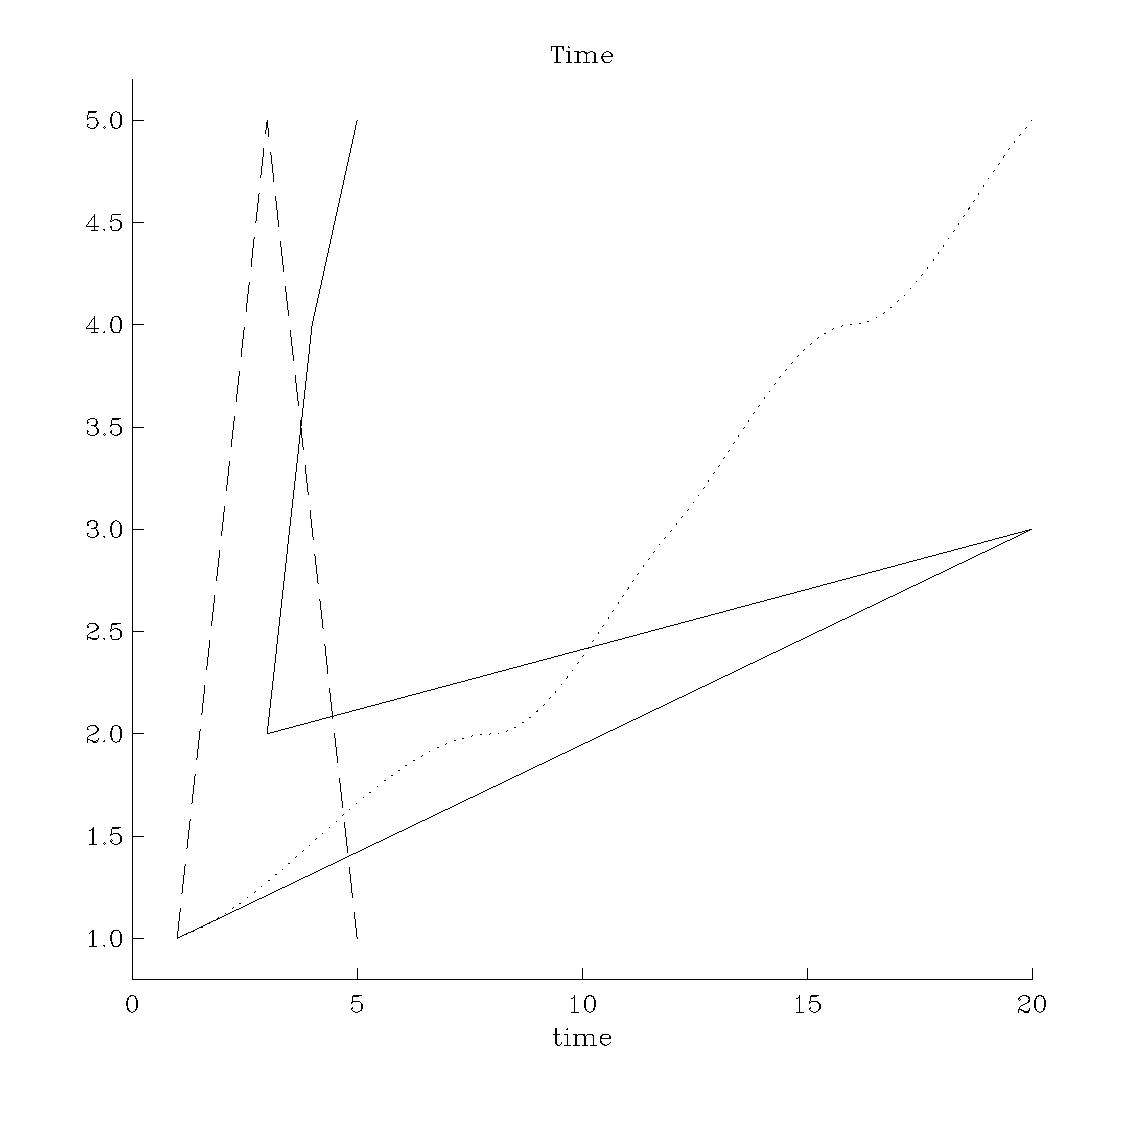
\includegraphics[width=4in]{gap3}
\caption{gap.ps}
\label{fig:gap.ps}
\end{center}
\end{figure}
\begin{figure}[htbp]
\begin{center}
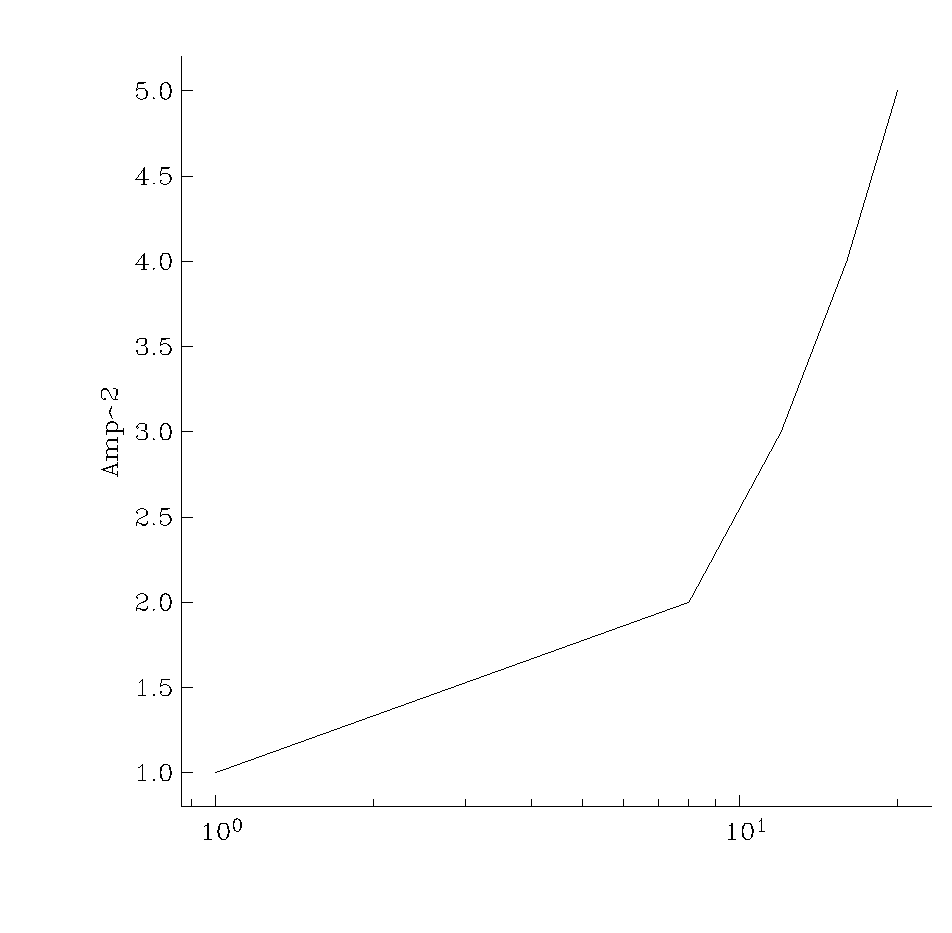
\includegraphics[width=4in]{gap4}
\caption{gap2.ps}
\label{fig:gap2.ps}
\end{center}
\end{figure}

\begin{figure}[htbp]
\begin{center}
\includegraphics[width=4in]{gap5}
\caption{newplot.ps}
\label{fig:newplot.ps}
\end{center}
\end{figure}

\end{document} 